\documentclass{article}
\usepackage{graphicx}
\usepackage{pdfpages}
\usepackage[moderate]{savetrees}
\begin{document}
% Research into:
% - Eigenfaces
% - Sparse Low Rank Bilinear Discriminative Model
% - What are liveness tests
% - How can we test a system that we create?
% - What test data is available? ROSE-Youtu Face liveness detection dataset
% - Deep Learning based face liveness detection in videos
% - Cameras used: mobile cameras (most methods use average resolution images from webcams or camera phone)
% - "Deep learning based face liveness detection in videos" https://ieeexplore.ieee.org/document/8090202/
% - Ideas: texture based - an image of a face will have the facial textures, while the texture of a piece of paper is very different.
% - Video vs Photo. Wtih a video, you don't just use the subject image, but also factor in movement and changes.
    
    \paragraph{Title}
        Facial Liveness Testing - an analysis of different methods
    \paragraph{Project Type}
        Computer Vision, Image Processing and Security
    \paragraph{Description}
        - In order to avoid spoofing in facial recognition systems, liveness tests are needed.
        - There are many facial liveness tests, but a comparison of these methods against one another doesn't currently exist.
    \paragraph{Preliminary Preparation}
        \begin{itemize}
            - Existing liveness tests
            - What are the datasets available for testing/training of these liveness methods?
        \end{itemize}
    \paragraph{Minimum Objectives}
        \begin{itemize}
            - 
        \end{itemize}
    \paragraph{Intermediate Objectives}
        \begin{itemize}
          - 
        \end{itemize}
    \paragraph{Advanced Objectives}
        \begin{itemize}
         - Implement facial flashing
        \end{itemize}
    \paragraph{References}
        \begin{itemize}
            \item Keras (https://keras.io) for Machine Learning
            \item OpenCV (https://opencv.org/) for Image Processing
        \end{itemize}

   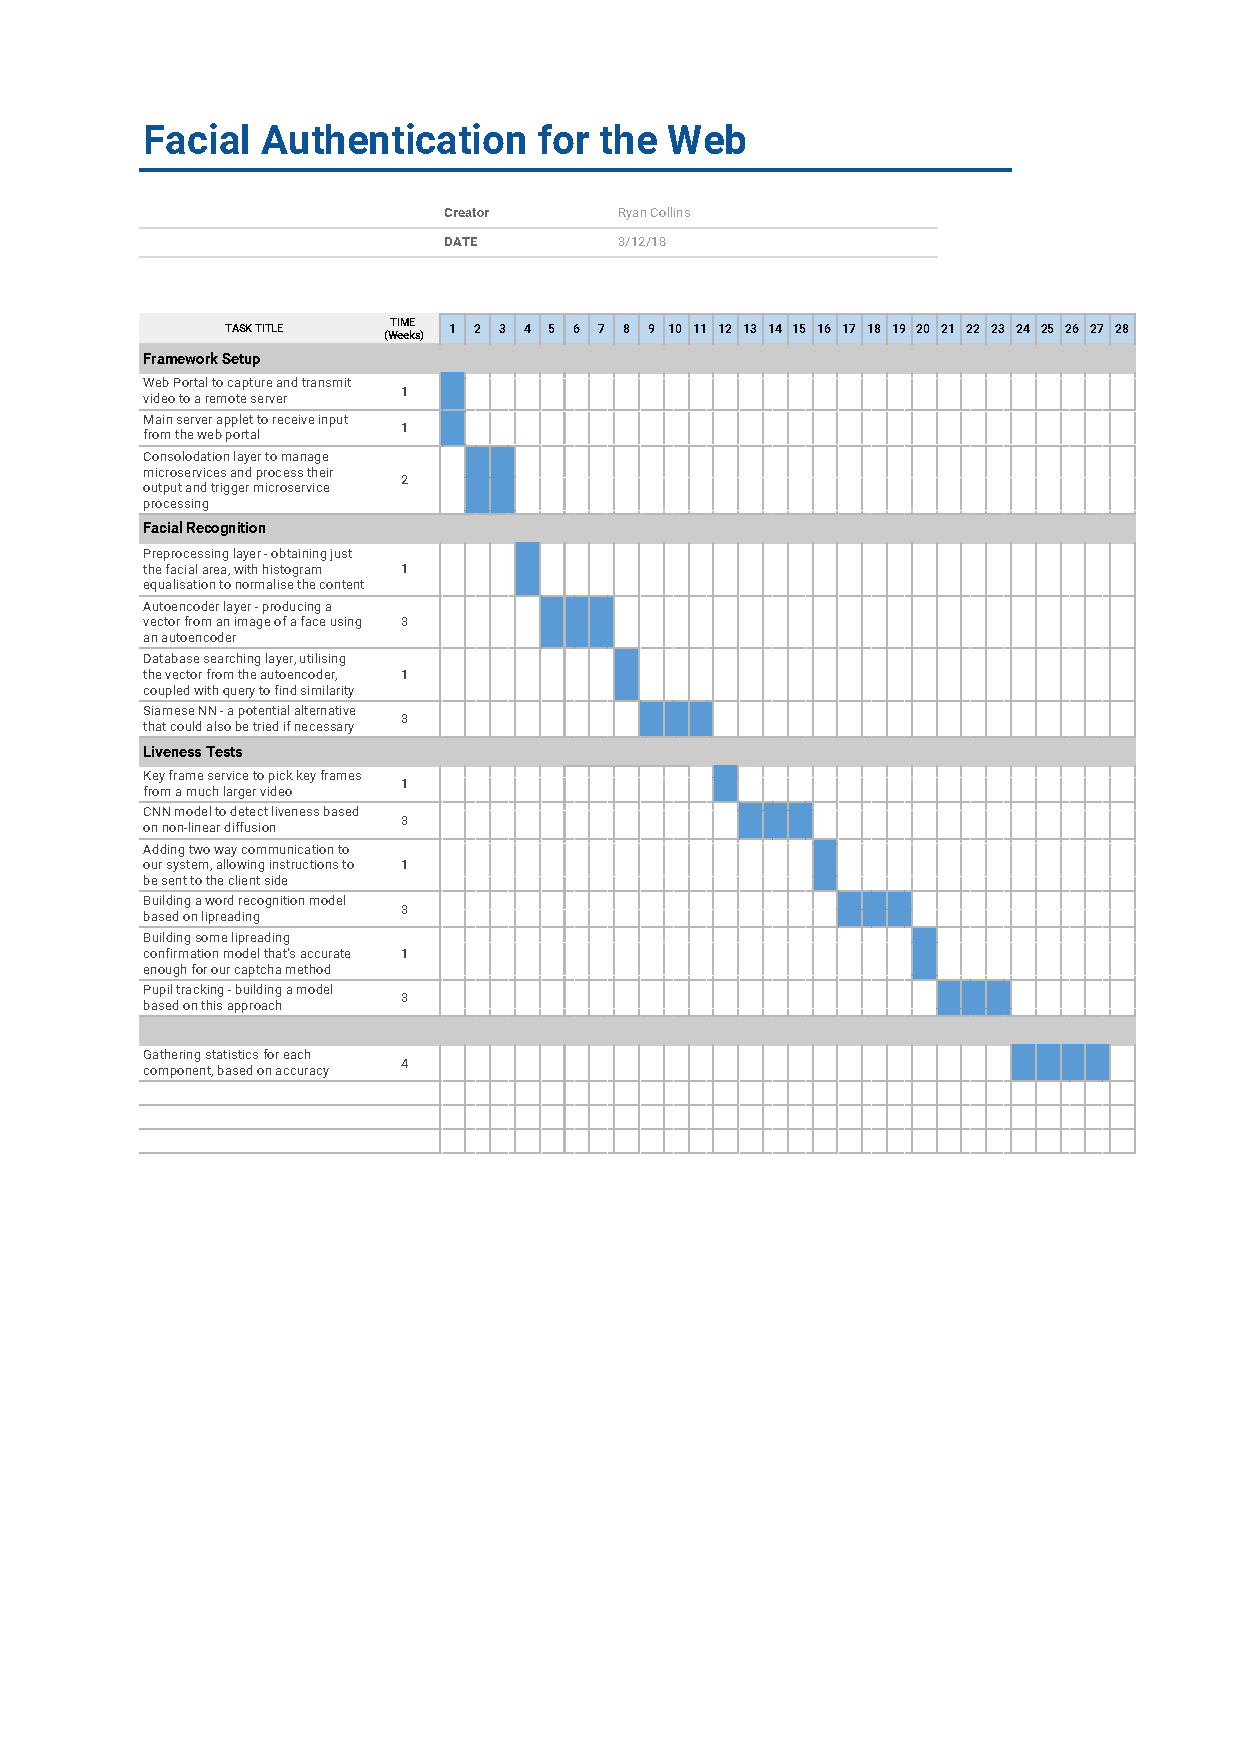
\includepdf{gantt.pdf}
\end{document}